\documentclass[12pt,a4paper]{article}
\usepackage[utf8]{inputenc}
\usepackage{graphicx}
\usepackage{tikz}
\usetikzlibrary{fit}
\usepackage{lmodern}
\usepackage{sectsty}


\sectionfont{\color{cyan}}

\begin{document}
   \begin{titlepage}
      {\fontfamily{lmss}\selectfont
      	\centering
      	
\includegraphics[width=0.30\textwidth]{logo.png}\par\vspace{1cm}
      	{\LARGE Compiax \par}
      	\vspace{0.25cm}
      	{\huge\bfseries \color{cyan}SplitBill\par}
      	\vspace{1cm}
      	{\Large\textit{by} Brute Force\par}
         \vspace{0.25cm}
         \begin{tikzpicture}
            \node [inner sep=0pt,,outer sep=0pt,clip,rounded corners=0.5cm] (pict) at (0,0) {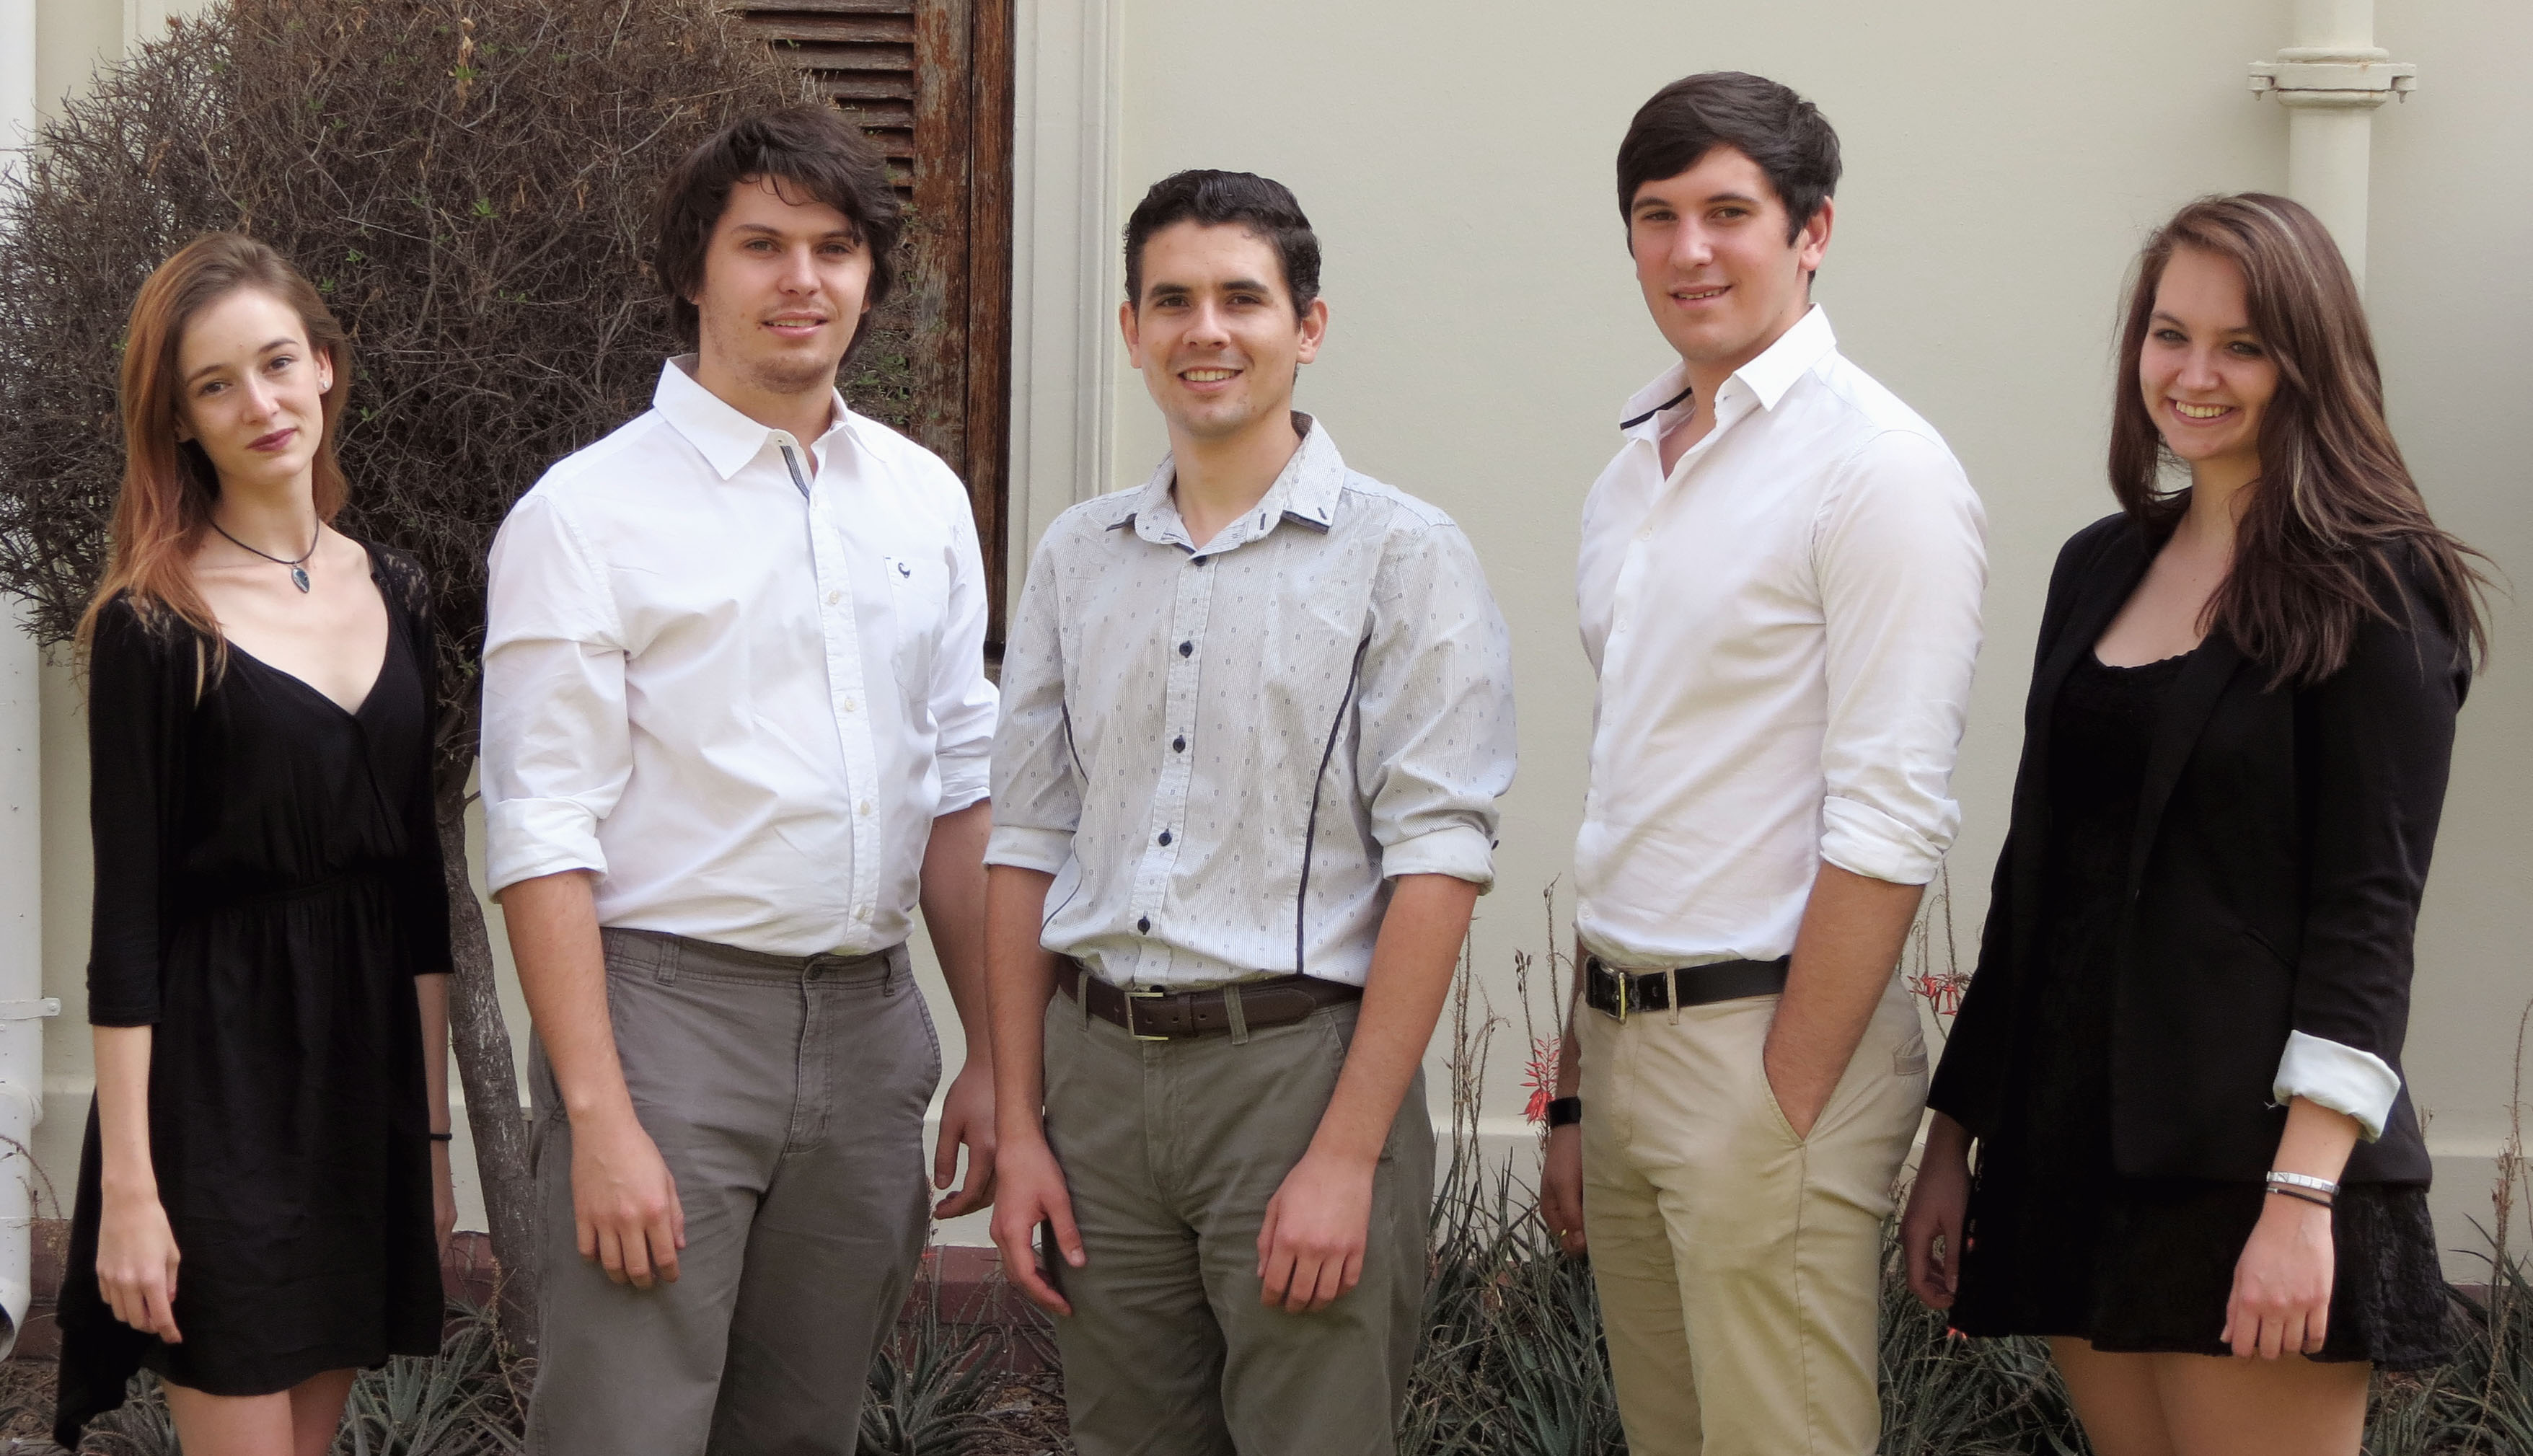
\includegraphics[width=0.9\textwidth]{team.jpg}};
            \node[fit=(pict),rounded corners=.55cm,inner sep=2pt]{};
         \end{tikzpicture}

         \par\vspace{1cm}
         \date{}
         \author{}
         \title{}
         \centering
         \textbf{Authors:}\\
         Mia Gerber\\
         Matthew Perry\\
         Wanrick Willemse\\
         Duart Breedt\\
         Linda Potgieter\\
      }
   \end{titlepage}
   \maketitle
   \tableofcontents
   \newpage

   \section{Introduction}
   The project presented is the development of a mobile application that will manage the division of items on a restaurant bill among the patrons around the table. This document serves as our proposal of how to address this issue.

   \section{The Project}
   At the highest level our objective is to create a user friendly app, that is visually appealing and enjoyable to use. The specifications determined that:
   \begin{itemize}
      \item \textbf{Capture and interpret the bill}\\
      Here ellaborate
      \item \textbf{Add users}\\
      Here ellaborate
      \item \textbf{Provide an interface}\\
      Here ellaborate
      \item \textbf{Live sync}\\
      Here ellaborate
      \item \textbf{Learn}\\
      Here ellaborate
      \item \textbf{App and server}\\
      Here ellaborate
   \end{itemize}
   Additionally we thought

   \section{Development Methodologies}
   Some Scrum, Some agile

   \section{Our Team}
   Team details here:
   Brute Force is a ragtag team of stalwart friends, off on a whirlwind big city adventure.
\end{document}
